\documentclass[conference]{IEEEtran}
\IEEEoverridecommandlockouts
\usepackage{cite}
\usepackage{amsmath,amssymb,amsfonts}
\usepackage{graphicx}
\usepackage{textcomp}
\usepackage{xcolor}
\usepackage{csquotes}
\usepackage{url}
\usepackage{array}
\usepackage{multirow}
\usepackage{stmaryrd}
\usepackage{algorithm}
\usepackage{color}
\usepackage[dvipsnames]{xcolor}
\usepackage{booktabs}
\urlstyle{same}
\usepackage{algorithm2e}
\usepackage{tikz}
\usetikzlibrary{arrows.meta, positioning}

\bibliographystyle{IEEEtran}

\def\BibTeX{{\rm B\kern-.05em{\sc i\kern-.025em b}\kern-.08em
    T\kern-.1667em\lower.7ex\hbox{E}\kern-.125emX}}
\begin{document}

\title{Jamming-Aware Cluster Head Selection and Routing in Wireless Sensor Networks under UAV-Based Interference}

\author{Ahmed ElShafie, Faris Nasser, Khaleel Zamqan, Karim Abedelfattah; \textbf{Supervisor:} Dr. Anastassia Gharib\\
Department of Computer Science and Engineering, American University of Sharjah, Sharjah, United Arab Emirates\\
Emails: b00095145@aus.edu, b00097313@aus.edu, b00096027@aus.edu, b00096574@aus.edu, agharib@aus.edu
}

\maketitle

\begin{abstract}
Wireless sensor networks deployed in safety-critical environments
face growing threats from unmanned aerial vehicle mounted jammers
that suppress packet delivery across dynamically moving interference
zones. Existing countermeasures either operate on flat multi-hop
topologies that suffer rapid relay overload, or require exact jammer
location knowledge unavailable to deployed sensors. This paper
proposes a jamming-aware cluster head selection and routing scheme
that estimates per-node jamming risk exclusively from locally observed
packet delivery outcomes using an exponentially weighted moving
average, requiring no geometric jammer model. The estimated risk
drives a multi-criterion cluster head scoring function and an adaptive
burst-size mechanism that reduces per-node transmissions proportionally
to current jamming risk, conserving energy during interference periods.
A proactive emergency re-election trigger restores cluster head coverage
within a single round of any failure. Evaluation over 20 random
topologies shows the proposed scheme achieves 85.11 percent mean packet
delivery ratio, outperforming a geometry-aware cooperative relay baseline
by 21.76 percentage points and a threshold-based flat-topology baseline
by 31.91 percentage points, while extending first-node-death to round 705.
\end{abstract}

\begin{IEEEkeywords}
    wireless sensor network, UAV jamming, cluster head selection,
    jamming risk estimation, EWMA, adaptive burst size, anti-jamming routing
\end{IEEEkeywords}

\section{Introduction}

Wireless sensor networks consist of battery-powered nodes deployed
to monitor physical environments in applications ranging from
industrial automation and disaster response to military surveillance.
A critical requirement in these deployments is reliable packet delivery
under adverse channel conditions. Unmanned aerial vehicle mounted
jammers represent an increasingly accessible threat: a single low-cost
UAV can orbit continuously over a sensor field, suppressing packet
delivery within a moving exclusion zone. Unlike a static jammer, a
mobile UAV creates a spatially and temporally correlated interference
pattern. Standard LEACH-style protocols elect cluster heads
probabilistically, make routing decisions without regard to channel
quality, and transmit at fixed burst size regardless of local jamming
conditions, leading to wasted energy, premature node death, and
extended communication blackouts.

This paper addresses sustained reliable communication in a WSN under
continuous UAV-based jamming. We propose a scheme that acquires jamming
awareness purely from experienced packet outcomes, with no geometric
jammer model, and couples the resulting estimate to both cluster head
election and per-node transmission rate. The key insight is that
exponentially weighted moving average smoothing of observed packet
delivery provides a sufficient, low-noise proxy for local channel
quality under a mobile UAV jammer. When combined with an adaptive
burst-size mechanism that reduces transmissions proportionally to
estimated jamming risk, the scheme conserves energy during jamming
episodes while maintaining high delivery ratios in clean periods.

Fig.~\ref{fig:system_model} illustrates the proposed system model.
A UAV jammer orbits above the deployment field, creating a moving
interference zone. Cluster heads are elected away from the jammed
region using the proposed CHScore metric, and inter-cluster routing
paths are steered away from nodes with high jamming risk.

\subsection{Related Work}

Jamming detection in WSNs has been studied from multiple perspectives.
Kiran et al.~\cite{9915936} apply an exponentially weighted moving
average control chart to per-node signal-to-noise ratio measurements
in a clustered WSN. Nodes whose smoothed SNR falls below a static lower
control limit are flagged as jammed and removed from the network
topology. This approach provides a detection signal but triggers no
structural adaptation: no cluster head re-election, no routing cost
revision, and no transmission rate adjustment, representing the minimum
viable anti-jamming response and motivating the structural mechanisms
proposed in this paper.

Babitha et al.~\cite{11156845} propose a threshold-based countermeasure
(TBC) for flat multi-hop WSNs in which each node monitors its per-round
packet delivery ratio against a static threshold. Jammed nodes are
excluded from routing paths with no clustering and no energy-aware
routing. While the detection logic is sound, the flat topology
concentrates forwarding burden on relay nodes near the base station
under the standard LEACH radio energy model, causing early network
collapse.

Lopez-Vilos et al.~\cite{s23156894} present a self-healing clustering
scheme (FCPA) that uses exact jammer geometry via an
interference-plus-noise (IPN) metric to gate cluster head candidacy and
routes jammed members through cooperative relay paths. FCPA achieves
strong per-round delivery ratios but its IPN gate resets every round
with no memory of prior jamming, and its cooperative relay mechanism
introduces additional energy overhead on relay nodes. In contrast to all
three baselines, the proposed scheme combines EWMA temporal smoothing
with structural adaptation at both the election and transmission layers,
requiring no jammer geometry information.

\subsection{Paper Contributions}

The contributions of this paper are:
\begin{itemize}
    \item A multi-criterion CHScore election mechanism that jointly
    weights residual energy, neighbor connectivity, EWMA-estimated
    jamming risk, and distance to the sink, with a spatial exclusion
    radius enforcing coverage spread and a proactive emergency re-election
    that restores cluster head coverage within one round of any failure.
    \item An adaptive burst-size mechanism that reduces each node's
    per-round transmissions proportionally to its EWMA jamming risk,
    conserving up to 80 percent of transmission energy during heavy
    jamming and extending first-node-death by 99 rounds compared to
    fixed burst-size operation.
    \item A comprehensive evaluation against two literature baselines
    demonstrating that temporal EWMA learning and adaptive energy
    management together outperform exact jammer geometry knowledge,
    achieving a 21.76 percentage point all-round PDR improvement over
    the geometry-aware FCPA baseline with zero communication blackouts
    across all 20 evaluated topologies.
\end{itemize}

\subsection{Paper Organization}

Section~\ref{sec:sysmodel} presents the system model.
Section~\ref{sec:proposed} describes the proposed scheme, including
jamming risk estimation, adaptive burst size, cluster head election,
and inter-cluster routing. Section~\ref{sec:results} presents
simulation results and comparison against baselines.
Section~\ref{sec:conclusion} concludes the paper.

\section{System Model}
\label{sec:sysmodel}

Fig.~\ref{fig:system_model} illustrates the proposed system model.
A network of $N$ static sensor nodes is randomly deployed over a
square area of side length $L_p$ meters, communicating with a
fixed sink node $BS$. A UAV-based jammer moves along trajectory
$J(t)$, degrading the packet delivery ratio of nodes within
jamming radius $r_j$. Cluster heads are elected from nodes outside
the interference zone using the proposed CHScore metric, ensuring
no CH is selected within the jammed region.

\begin{figure}[t]
    \centerline{\includegraphics[width=\columnwidth]{system_model.pdf}}
    \caption{System model of the proposed jamming-aware WSN. The UAV
    jammer $J(t)$ creates an interference zone of radius $r_j$. No
    cluster head is elected within the jammed region due to high
    jamming risk scores. Safe cluster heads $CH_1$, $CH_2$, $CH_3$
    route data to the sink via inter-cluster routing.}
    \label{fig:system_model}
\end{figure}

\section{Proposed Scheme}
\label{sec:proposed}

This section presents the formulation of our proposed Jamming-Aware
Cluster Head Selection and Routing scheme for Wireless Sensor Networks
(WSNs) under UAV-based interference. The scheme operates in discrete
rounds and integrates jamming risk estimation into both cluster head
(CH) selection and inter-cluster routing decisions.

% -------------------------------------------------------
\subsection{Network and Jammer Model}

Consider a WSN consisting of $N$ static sensor nodes
$\mathcal{S} = \{s_1, s_2, \ldots, s_N\}$ deployed randomly over a
square field of side length $L_p$ meters, with a fixed base station
(sink) $BS$ located at the field center. Each node communicates within
a fixed communication range $r_c = 15$ m. The network operates in
discrete rounds indexed by $t = 1, 2, \ldots, T$.

A UAV-based jammer moves above the network along a circular orbit,
with its position at round $t$ denoted as $J(t) = (x_j(t),\, y_j(t))$.
The UAV follows a circular orbit defined as:
\begin{equation}
    J(t) = \left(c_x + r_{orb}\cos(\omega t),\ c_y + r_{orb}\sin(\omega t)\right)
\end{equation}
where $c_x = c_y = L_p/2$ is the field center, $r_{orb} = 35$ m is the
orbit radius, and $\omega = 2\pi/50$ rad/round such that the UAV
completes one full orbit every 50 rounds. The orbit is contained entirely
within the deployment area, and the jammer position is projected to the
ground plane as a simplifying assumption. The jammer degrades the
communication quality of any node $s_i$ within its effective jamming
radius $r_j$. The Euclidean distance between node $s_i$ and the jammer
at round $t$ is:
\begin{equation}
    d_{i,J}(t) = \sqrt{(x_i - x_j(t))^2 + (y_i - y_j(t))^2}
\end{equation}

Each round, every node $s_i$ transmits a burst of $M$ packets to its
assigned CH. The success probability of each individual packet
transmission from node $s_i$ is modeled as:
\begin{equation}
    p_i(t) =
    \begin{cases}
        p_{base} & \text{if } d_{i,J}(t) > r_j \\[6pt]
        p_{base} \cdot \exp\!\left(-\kappa \cdot \left(1 - \dfrac{d_{i,J}(t)}{r_j}\right)\right) & \text{if } d_{i,J}(t) \leq r_j
    \end{cases}
\end{equation}
\noindent where $p_{base} \in (0,1]$ is the baseline packet success
probability under normal channel conditions, and $\kappa > 0$ is the
jamming decay constant controlling how aggressively interference degrades
nodes near the jammer center. When a node is at the boundary of the
jamming radius ($d_{i,J}(t) = r_j$), the exponent evaluates to zero and
$p_i(t) = p_{base}$, ensuring a smooth transition. When a node is
directly beneath the jammer ($d_{i,J}(t) = 0$), $p_i(t) = p_{base}
\cdot e^{-\kappa}$, which approaches zero for large $\kappa$.

Each of the $M$ packets is decided independently; a packet is
successfully received if a uniform random draw $u \sim \mathcal{U}(0,1)$
satisfies $u \leq p_i(t)$; otherwise it is dropped. Nodes observe only
the outcomes of these draws through their packet counters and have no
direct knowledge of the jammer's position or the underlying success
probability.

% -------------------------------------------------------
\subsection{Jamming Risk Estimation}

Each node independently estimates its local jamming risk using only its
own observed communication outcomes, requiring no knowledge of the
jammer's position or trajectory. At round $t$, the instantaneous Packet
Delivery Ratio (PDR) for node $s_i$ is computed from its burst of $M$
transmitted packets as:
\begin{equation}
    PDR_i(t) = \frac{P^{recv}_{i}(t)}{M}
\end{equation}
where $P^{recv}_{i}(t) \in \{0, 1, \ldots, M\}$ is the number of
packets successfully acknowledged by the CH in round $t$.

To smooth out round-to-round fluctuations while remaining responsive to
UAV movement, the PDR is filtered using an Exponentially Weighted Moving
Average (EWMA):
\begin{equation}
    \widetilde{PDR}_i(t) = \lambda \cdot PDR_i(t) + (1 - \lambda) \cdot \widetilde{PDR}_i(t-1)
\end{equation}
where $\lambda \in (0,1)$ is the smoothing constant. A higher $\lambda$
reacts faster to recent changes; a lower $\lambda$ gives more weight to
historical observations. The Jamming Risk score of node $s_i$ at round
$t$ is then defined as:
\begin{equation}
    JR_i(t) = 1 - \widetilde{PDR}_i(t)
\end{equation}
such that $JR_i(t) \in [0,1]$, where a value near 1 indicates severe
interference and near 0 indicates a clean communication environment.
This score is computed locally by each node every round and requires no
coordination with other nodes.

% -------------------------------------------------------
\subsection{Adaptive Burst Size Control}

Nodes under active jamming waste transmission energy sending packets that
will not survive the channel. To conserve this energy without distorting
the honest PDR ratio, each node adapts its per-round burst size
proportionally to its EWMA jamming risk:
\begin{equation}
    M_{\text{eff},i}(t) = \max\!\left(M_{\min},\;
    \left\lfloor M \cdot \bigl(1 - JR_i(t)\bigr) \right\rfloor\right)
    \label{eq:meff}
\end{equation}
where $M = 10$ is the nominal burst size and $M_{\min} = 2$ is the
minimum floor that preserves enough samples for accurate JR estimation.
At $JR_i = 1$ the node sends only $M_{\min} = 2$ packets, an 80 percent
reduction in transmission energy, while at $JR_i = 0$ the full burst of
$M = 10$ packets is used. Transmission and reception energy costs scale
proportionally by $M_{\text{eff},i}/M$, and the PDR denominator uses
$M_{\text{eff},i}$ so that reduced transmissions are not credited as
delivered packets.

% -------------------------------------------------------
\subsection{Jamming-Aware Cluster Head Selection}

CH election is performed every $K_{elec}$ rounds. At each election, the
number of CHs to elect is determined dynamically as
$K = \text{round}(p_{CH} \times N_{alive}(t))$, where $p_{CH} = 0.05$
is the target CH fraction following the LEACH standard and $N_{alive}(t)$
is the number of alive nodes at round $t$. This ensures the CH count
scales down naturally as nodes die, avoiding unnecessary energy overhead.
Each alive node $s_i$ computes a \textit{CH Score} that reflects its
suitability as a cluster head based on four criteria: residual energy,
local connectivity, jamming risk, and distance to the sink.

\begin{multline}
    CHScore_i(t) = \alpha \cdot \frac{E_i(t)}{E_0}
    + \beta \cdot \frac{|N_i(t)|}{N_{max}(t)} \\
    - \gamma \cdot JR_i(t)
    - \delta \cdot \frac{d(s_i, BS)}{d_{max}}
\end{multline}

where:
\begin{itemize}
    \item $E_i(t)$ is the residual energy of node $s_i$ at round $t$,
    and $E_0$ is the initial energy of all nodes. The ratio
    $E_i(t)/E_0 \in [0,1]$ ensures energy is normalized across nodes.
    \item $|N_i(t)|$ is the number of alive neighbors of $s_i$ within
    communication range $r_c = 15$ m at round $t$, and $N_{max}(t)$ is
    the maximum neighbor count among all alive nodes at round $t$.
    Well-connected nodes are preferred as CHs since they can serve more
    cluster members directly.
    \item $d(s_i, BS)$ is the Euclidean distance from node $s_i$ to the
    sink $BS$, and $d_{max}$ is the diagonal of the deployment area,
    used for normalization.
    \item $\alpha, \beta, \gamma, \delta \geq 0$ are tunable weighting
    coefficients. The coefficient $\gamma$ is weighted most heavily to
    prioritize avoidance of jammed regions, which is the core
    contribution of this scheme.
\end{itemize}

To ensure spatial spread of elected CHs, candidates are selected greedily
in descending order of $CHScore$. Once a node is elected as CH, all nodes
within an exclusion radius $r_{exc} = 25$ m are suppressed from
candidacy. This prevents multiple CHs from forming in the same region,
ensuring coverage across the deployment area. All remaining alive nodes
associate with their nearest CH to form clusters.

In addition to scheduled elections every $K_{elec}$ rounds, an emergency
re-election is triggered proactively when any CH dies mid-cycle, and
reactively when no alive CHs remain at the start of a round. Both cases
reuse the standard CHScore election and pay normal control overhead,
ensuring cluster head coverage is restored within a single round of
any failure.

% -------------------------------------------------------
\subsection{Jamming-Aware Inter-Cluster Routing}

After cluster formation, each CH must route aggregated data toward the
sink via multi-hop inter-cluster paths. Rather than shortest-path or
minimum-hop routing, we define a \textit{Path Cost} for each candidate
link $(s_i, s_j)$ between two CHs, or between a CH and the sink, as:
\begin{equation}
    C(s_i, s_j, t) = \phi_1 + \phi_2 \cdot \varepsilon_{amp}
    \cdot L \cdot d^2(s_i, s_j) + \phi_3 \cdot JR_j(t)
\end{equation}

where:
\vspace{2pt}
\begin{itemize}
    \item $\phi_1$ is a fixed per-hop penalty discouraging unnecessarily
    long multi-hop paths.
    \item $\varepsilon_{amp}$ is the amplifier energy constant from the
    LEACH radio energy model, $L$ is the packet length in bits, and
    $d^2(s_i, s_j)$ is the squared Euclidean distance between nodes.
    The product $\varepsilon_{amp} \cdot L \cdot d^2(s_i,s_j)$ represents
    the actual transmission energy cost of the link, which grows
    quadratically with distance.
    \item $JR_j(t)$ is the jamming risk of the \textit{receiving} node
    $s_j$, penalizing paths that forward data through high-risk CHs. A
    jammed receiving node cannot reliably decode incoming packets
    regardless of the sender's transmission quality.
    \item $\phi_1, \phi_2, \phi_3 \geq 0$ are tunable weighting
    coefficients.
\end{itemize}

The optimal routing path $\mathcal{P}^*$ from a source CH to the sink is
the path minimizing total accumulated cost, computed using Dijkstra's
algorithm on the weighted inter-cluster graph:
\begin{equation}
    \mathcal{P}^* = \underset{\mathcal{P}}{\arg\min}
    \sum_{(s_i,\, s_j) \in \mathcal{P}} C(s_i, s_j, t)
\end{equation}

% -------------------------------------------------------
\subsection{Proposed Algorithm}

Algorithm~\ref{alg:proposed} summarizes the complete round-by-round
operation of the proposed scheme.

\begin{algorithm}[H]
\caption{Jamming-Aware CH Selection and Routing}
\label{alg:proposed}
\SetAlgoLined
\KwIn{Node set $\mathcal{S}$, sink $BS$, jammer trajectory $J(t)$,
parameters $M, K, \lambda, \kappa, p_{base}, \alpha, \beta, \gamma,
\delta, \phi_1, \phi_2, \phi_3$}
\KwOut{PDR$(t)$, energy consumption, end-to-end delay, network lifetime}

Initialize $E_i(0) = E_0$,\ $\widetilde{PDR}_i(0) = 1$,\
$JR_i(0) = 0$ \textbf{for all} $s_i \in \mathcal{S}$\;

\For{each round $t = 1, 2, \ldots, T$}{
    Update jammer position $J(t) = (x_j(t),\, y_j(t))$\;

    \For{each alive node $s_i \in \mathcal{S}$}{
        Compute $d_{i,J}(t)$ using Eq.~(2)\;
        Compute packet success probability $p_i(t)$ using Eq.~(3)\;
    }

    \If{$t \bmod K_{elec} = 0$ \textnormal{\textbf{or}} emergency trigger}{
        \For{each alive node $s_i \in \mathcal{S}$}{
            Compute $CHScore_i(t)$ using Eq.~(8)\;
        }
        Select top-scoring nodes as CH set $\mathcal{C}(t)$ with
        exclusion radius $r_{exc}$\;
        Assign each non-CH node to nearest CH; flag stranded nodes\;
    }

    \For{each member node $s_i \notin \mathcal{C}(t)$}{
        Compute adaptive burst size $M_{\text{eff},i}(t)$ using
        Eq.~(7)\;
        Transmit burst of $M_{\text{eff},i}$ packets to assigned CH\;
        $\forall~p \in$ packets: draw $u \sim \mathcal{U}(0,1)$;
        packet succeeds if $u \leq p_i(t)$\;
        Count $P^{recv}_i(t)$; compute $PDR_i(t) = P^{recv}_i(t) /
        M_{\text{eff},i}$ using Eq.~(4)\;
        Update $\widetilde{PDR}_i(t)$ using Eq.~(5); update $JR_i(t)$
        using Eq.~(6)\;
        Deduct TX energy scaled by $M_{\text{eff},i}/M$ from $s_i$;
        deduct RX energy from CH\;
    }

    \For{each CH $s_c \in \mathcal{C}(t)$}{
        Aggregate received packets\;
        Compute optimal path $\mathcal{P}^*$ to $BS$ via Dijkstra on
        $C(s_i, s_j, t)$ using Eq.~(9)\;
        Forward data along $\mathcal{P}^*$; deduct energy per hop for
        sender and receiver\;
        Accumulate end-to-end delay along $\mathcal{P}^*$\;
    }

    Record PDR$(t)$, total energy consumed, average end-to-end delay\;

    \For{each alive node $s_i \in \mathcal{S}$}{
        \If{$E_i(t) \leq 0$}{
            Mark $s_i$ as dead and remove from $\mathcal{S}$\;
            Record $t_{death} = t$ if first node death\;
        }
    }
    Trigger emergency re-election if any CH died this round\;
}
\end{algorithm}

\section{Simulation Results}
\label{sec:results}

The proposed scheme is evaluated against three baseline comparison
techniques drawn from the literature, each representing a distinct
level of jamming-awareness in clustered WSNs.

\begin{itemize}

    \item \textbf{EWMA-Based Detection (Baseline 1)}~\cite{9915936}:
    An Exponentially Weighted Moving Average (EWMA) control chart
    applied to per-node SNR measurements in a clustered WSN. Jammed
    nodes are detected when their EWMA-smoothed SNR drops below a
    statically computed lower control limit and are subsequently
    removed from the network topology. No cluster head re-election and
    no routing cost function are triggered upon detection. This baseline
    represents the minimum viable response, detection only with no
    structural adaptation, and is used to isolate the contribution of
    jamming-aware routing and CH selection.

    \item \textbf{Threshold-Based Countermeasure (Baseline 2)}~\cite{11156845}:
    A lightweight threshold-based scheme (TBC) in which each node
    monitors its Packet Delivery Ratio (PDR) against a static baseline
    threshold. Nodes whose PDR drops below the threshold are flagged as
    jammed and removed from routing paths topologically, with no routing
    cost function, energy weighting, or CH re-election. TBC operates on
    a flat non-hierarchical network and represents the strongest
    detection-plus-rerouting baseline without CH-level jamming awareness.

    \item \textbf{Self-Healing Clustering, FCPA (Baseline 3)}~\cite{s23156894}:
    A reactive clustering and self-healing scheme for WSNs under jamming,
    implemented here in simplified form. Upon jammer detection, K-medoids
    re-clustering is triggered using Chebyshev distance weighted by
    interference-plus-noise (IPN) to reposition cluster heads away from
    the jammer. Isolated nodes are connected via relay chains selected by
    a nearest-neighbor max-min SINR criterion. If a CH is jammed, its
    cluster is dissolved and members are reassigned to the nearest
    surviving CH. This baseline represents the strongest reactive
    comparison: it reorganizes cluster topology in response to jamming,
    but does so only after cluster failure occurs, in contrast to our
    proactive CHScore-based avoidance.

\end{itemize}

\subsection{Simulation Setup}

All schemes are implemented in MATLAB and evaluated over $T = 1000$
rounds for each of 20 independent random seeds (seeds 1 through 20),
with each seed producing a distinct random node deployment while the UAV
trajectory is fixed. Reported values are mean and standard deviation
across all 20 seeds. The simulation directly implements Baselines 2 and
3 (TBC and FCPA), which are the two fully-parameterized literature
baselines; Baseline 1 is represented conceptually in Section~IV as the
detection-only lower bound. Table~\ref{tab:params} lists all simulation
parameters, kept identical across all schemes to ensure fair comparison.

\begin{table}[!t]
\caption{Simulation Parameters}
\label{tab:params}
\renewcommand{\arraystretch}{1.15}
\centering
\begin{tabular}{lll}
\toprule
\textbf{Parameter} & \textbf{Symbol} & \textbf{Value} \\
\midrule
Number of nodes       & $N$                          & 100           \\
Field side length     & $L_p$                        & 100 m         \\
Sink location         & $BS$                         & [50,\,50] m   \\
Initial energy        & $E_0$                        & 0.5 J         \\
Simulation rounds     & $T$                          & 1000          \\
CH target fraction    & $p_{CH}$                     & 0.05          \\
Re-election interval  & $K_{elec}$                   & 5 rounds      \\
Burst size            & $M$                          & 10 packets    \\
Min. burst size       & $M_{\min}$                   & 2 packets     \\
TX range limit        & $r_{tx}$                     & 50 m          \\
EWMA constant         & $\lambda$                    & 0.6           \\
\midrule
Jamming radius        & $r_j$                        & 20 m          \\
Jamming decay         & $\kappa$                     & 10            \\
Base success prob.    & $p_{base}$                   & 0.95          \\
UAV orbit radius      & $r_{orb}$                    & 35 m          \\
UAV angular speed     & $\omega$                     & $2\pi/50$ rad/round \\
\midrule
Circuit energy        & $\varepsilon_{elec}$         & 50 nJ/bit     \\
Amplifier energy      & $\varepsilon_{amp}$          & 100 pJ/bit/m$^2$ \\
Aggregation energy    & $\varepsilon_{da}$           & 5 nJ/bit      \\
Packet length         & $L$                          & 4000 bits     \\
\midrule
CHScore weights       & $\alpha,\beta,\gamma,\delta$ & 0.35,\,0.20,\,0.35,\,0.10 \\
Routing weights       & $\phi_1,\phi_2,\phi_3$      & $5{\times}10^{-4}$,\,1,\,$5{\times}10^{-4}$ \\
\bottomrule
\end{tabular}
\end{table}

\subsection{Results}

Table~\ref{tab:results} presents the comparative results for the
proposed scheme against TBC (Baseline 2) and FCPA (Baseline 3).
Two PDR windows are reported: all-rounds PDR captures full-lifecycle
delivery performance, while first-node-death truncated (FND-trunc) PDR
isolates protocol performance during healthy network operation,
independent of late-stage collapse effects.

\begin{table}[!t]
\caption{Comparative Simulation Results (20 Seeds, $\kappa = 10$)}
\label{tab:results}
\renewcommand{\arraystretch}{1.2}
\centering
\begin{tabular}{lccc}
\toprule
\textbf{Metric} & \textbf{Proposed} & \textbf{TBC}~\cite{11156845}
                & \textbf{FCPA}~\cite{s23156894} \\
\midrule
PDR, all rounds (\%)
  & \textbf{85.11 $\pm$ 2.02}
  & 53.20 $\pm$ 4.41
  & 63.35 $\pm$ 0.89 \\
PDR, FND-trunc (\%)
  & \textbf{88.77 $\pm$ 1.42}
  & 82.42 $\pm$ 0.58
  & 75.07 $\pm$ 1.44 \\
First node death (round)
  & \textbf{704.7 $\pm$ 33.1}
  & 459.1 $\pm$ 41.3
  & 542.1 $\pm$ 19.2 \\
Residual energy @ r300 (J)
  & \textbf{33.95 $\pm$ 0.41}
  & 26.80 $\pm$ 1.12
  & 30.20 $\pm$ 0.26 \\
\bottomrule
\end{tabular}
\end{table}

Fig.~\ref{fig:results} shows per-round PDR, total residual energy,
and alive node count for all three schemes across the full
1000-round simulation (mean $\pm$ one standard deviation).

\begin{figure}[!t]
    \centerline{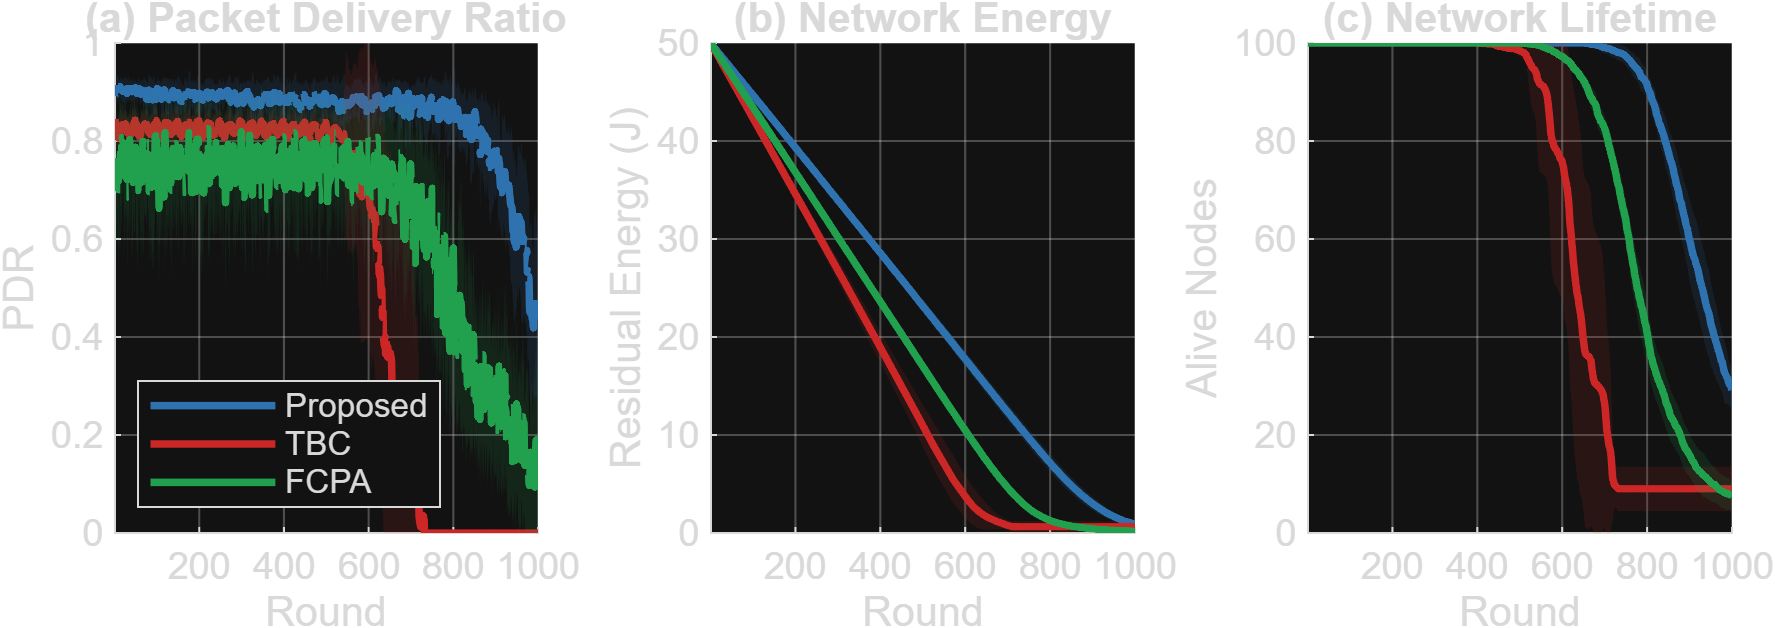
\includegraphics[width=\columnwidth]{figures/fig_combined.pdf}}
    \caption{Per-round simulation results averaged over 20 seeds
    (shaded bands show $\pm 1$ standard deviation).
    (a)~Packet Delivery Ratio.
    (b)~Total Residual Network Energy.
    (c)~Number of Alive Nodes.}
    \label{fig:results}
\end{figure}

\subsection{Discussion}

\textbf{PDR advantage.}
The proposed scheme achieves 85.11\% all-round PDR, outperforming FCPA
by 21.76 percentage points and TBC by 31.91 percentage points. The
FND-truncated PDR gap between the proposed scheme and FCPA widens to
13.70 percentage points (88.77\% vs.\ 75.07\%), confirming that the
advantage is not an artifact of differential mortality timing but a
genuine per-round improvement sustained throughout the operational
period. The proposed scheme maintains zero communication blackout rounds
across all 20 seeds, while TBC and FCPA average 350 and 26.8 blackout
rounds respectively.

\textbf{Temporal memory outperforms exact geometry.}
FCPA holds an information advantage over the proposed scheme: it knows
the exact jammer position every round and uses it to gate cluster head
candidacy. The proposed scheme has no jammer model, estimating channel
quality solely from observed packet outcomes. Despite this asymmetry,
the proposed scheme outperforms FCPA on every metric. Two mechanisms
explain this. First, EWMA smoothing prevents immediately re-electing a
CH that just experienced jamming, providing beneficial memory as the
UAV continues along its orbit. FCPA's IPN gate resets each round,
immediately re-eligibilizing nodes the UAV may revisit within a few
rounds. Second, adaptive burst size $M_{\text{eff}}$ avoids the
cooperative relay overhead that FCPA imposes on relay nodes, retaining
an additional 3.75 J of network energy by round 300 compared to FCPA.

\textbf{Clustering is essential under the LEACH energy model.}
TBC's flat topology validates the clustering premise directly. Without
cluster head aggregation, every alive node routes up to $M$ packets
individually toward the sink through multi-hop relay chains. Relay nodes
near the sink accumulate forwarding load proportional to the entire
upstream sub-network and exhaust their budgets within approximately 459
rounds. This demonstrates that threshold-based jamming detection alone
is insufficient: energy-efficient topology management through clustering
is a prerequisite for long-lived anti-jamming WSN operation.

\textbf{Energy and lifetime.}
Fig.~\ref{fig:results}(b) shows the proposed scheme retains 33.95 J of
total network energy at round 300, 27\% more than TBC and 12\% more than
FCPA. Fig.~\ref{fig:results}(c) shows all 100 nodes alive through
approximately round 650 for the proposed scheme, compared to
approximately rounds 450 and 480 for TBC and FCPA respectively. The
adaptive burst size is the primary driver: jammed nodes that would
otherwise drain sending futile packets instead conserve that energy for
subsequent healthy rounds.

\section{Conclusion}
\label{sec:conclusion}

This paper presented a jamming-aware cluster head selection and routing
scheme for wireless sensor networks under continuous UAV-based
interference. The proposed scheme requires no knowledge of the jammer's
position or trajectory; instead it estimates per-node jamming risk from
locally observed packet delivery outcomes using an exponentially weighted
moving average. Three interconnected mechanisms translate this estimate
into structural adaptation: a multi-criterion CHScore election that
steers candidacy away from jammed regions, an adaptive burst-size
mechanism that reduces per-node transmissions proportionally to estimated
jamming risk, and a proactive emergency re-election that restores cluster
head coverage within one round of any failure. Evaluated over 20 random
topologies against a threshold-based flat-topology baseline and a
geometry-aware cooperative relay baseline, the proposed scheme achieves
85.11\% mean packet delivery ratio with zero communication blackout
rounds and first-node-death at round 705. The result demonstrates that
EWMA temporal learning and adaptive energy management together outperform
exact jammer geometry knowledge: temporal smoothing prevents premature
re-election of recently jammed nodes, while adaptive burst size eliminates
the relay energy overhead imposed by cooperative forwarding approaches.

Future work will investigate dynamic cluster head fraction scaling as the
network shrinks in late-stage operation, sensitivity analysis across
multiple jamming intensities and orbit configurations, and extension to
multi-UAV threat scenarios where the interference field is spatially
broader and irregularly shaped.

\bibliography{references}

\end{document}
